\documentclass{article}
\usepackage[utf8]{inputenc}
\usepackage[T1]{fontenc}
\usepackage[francais]{babel}
\usepackage{lmodern}
\usepackage{graphicx}
\usepackage{geometry}

\geometry{hmargin=30pt, vmargin=30pt}

\title{Bilan mi-parcours : IHM Ecriture sur Tableau Virtuel}
\author{Bollini Kevin, Mélia Geoffrey, Pagès Julien, Saleil Baptiste}
\date{2 Mars 2012}

\begin{document}

\maketitle
	Nom du groupe : \textbf{PouerMouer}
	\section{Composition du groupe et contact}
	
	\begin{itemize}
	\item Kevin Bollini : kevin.bollini@etud.univ-montp2.fr \\
	\item Geoffrey Mélia : geoffrey.melia@etud.univ-montp2.fr \\
	\item Julien Pagès : julien.pages01@etud.univ-montp2.fr \\
	\item Baptiste Saleil : baptiste.saleil@etud.univ-montp2.fr \\
	\end{itemize} 	
	\section{Planning}
		\begin{center}
			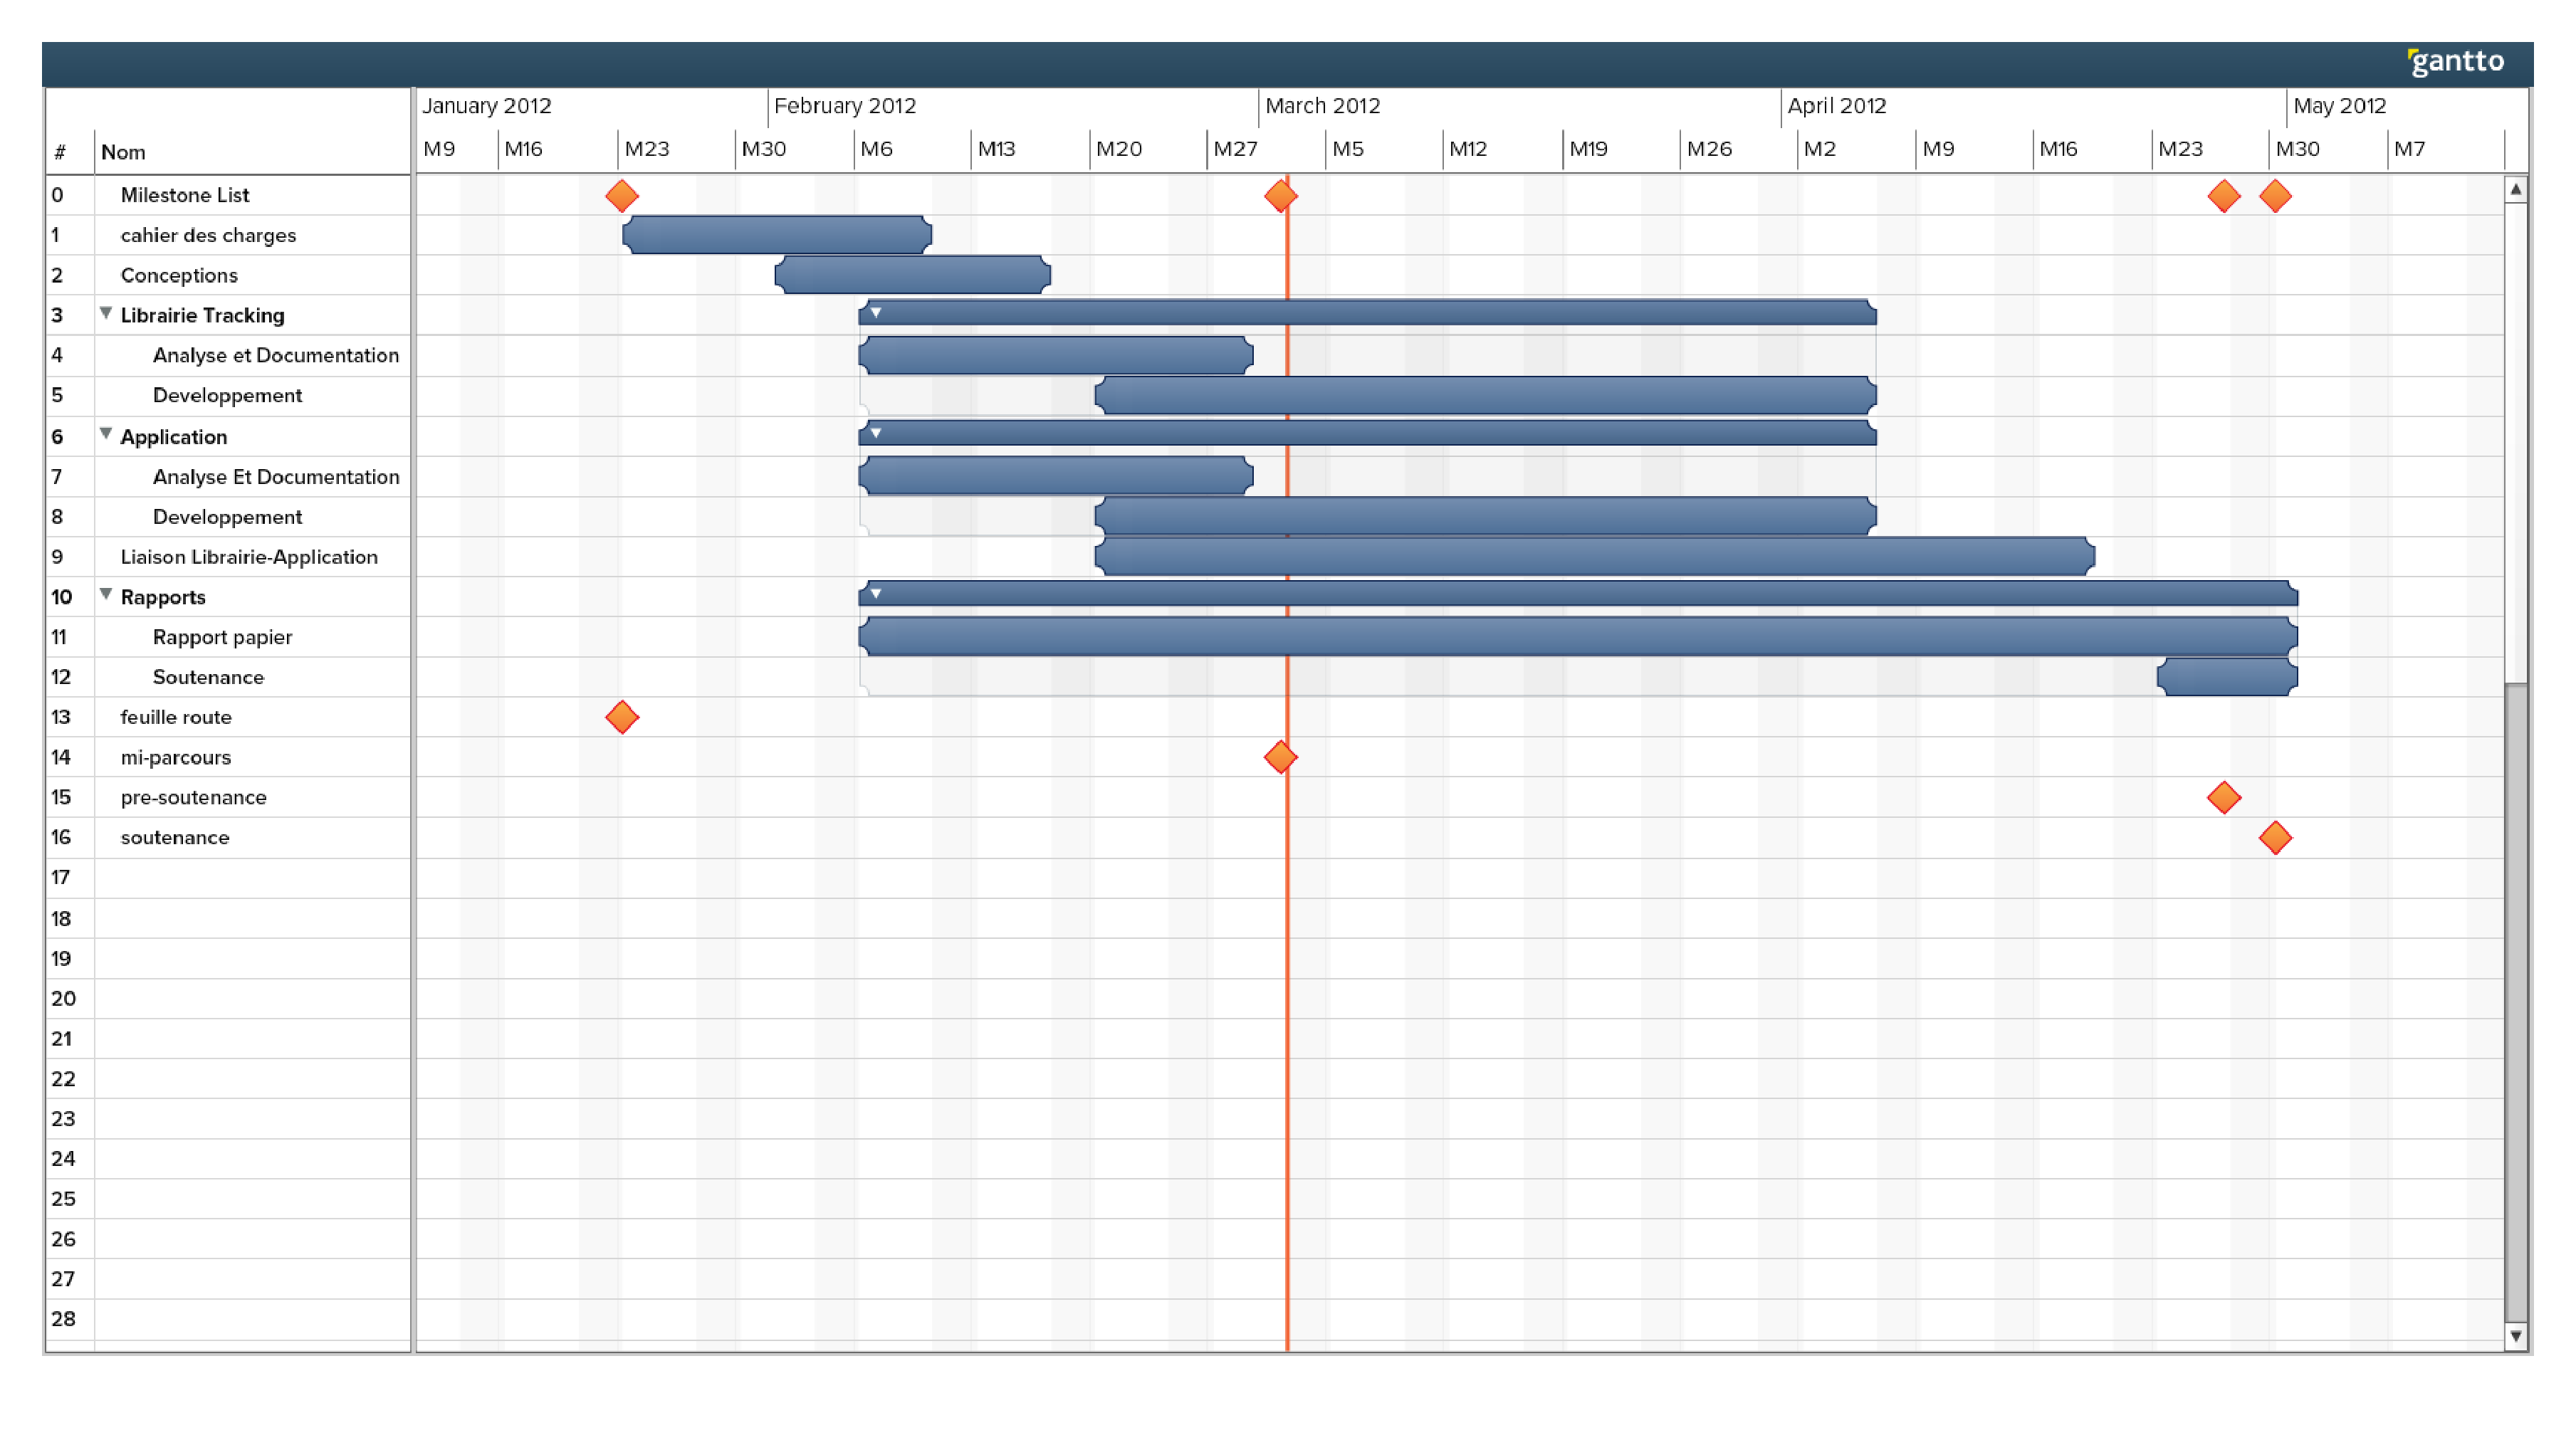
\includegraphics[scale=0.3]{retroplanning.pdf}
			\it rétro-planning, état actuel du projet
		\end{center}
	\section{Tâches effectuées}
		Une première version archaïque de l'application, permettant pour l'instant de réaliser une capture des mouvements d'un objet coloré et de les enregistrer sous forme de nuage de points sur le tableau blanc. \\
		Les deux sous-tâches ont été réalisées avec un temps effectif conforme à celui indiqué dans le planning initial et le cahier des charges, il est en revanche difficile de quantifier précisément le temps passé sur le projet. \\
		\subsection{Librairie}
		Cette partie a été réalisée par Kevin Bollini et Geoffrey Mélia. \\
			L'analyse et la conception de la librairie à été réalisée. Une première méthode de track naif par couleur à été implémentée et est utilisée par l'application. D'autre part, une méthode de track par forme est terminée mais n'est pas encore utilisable par l'application. 
		\subsection{Logiciel}
		Cette partie a été réalisée conjointement par Julien Pagès et Baptiste Saleil. \\
			L'analyse et la conception a été faite, un diagramme de classes UML et différents cas d'utilisations ont ainsi été réalisés. L'IHM du logiciel est donc globalement en place, nous avons la possibilité de choisir la webcam à utiliser, de l'étalonner suivant une couleur, et de reconnaître les mouvements via la librairie. \\
			Il y a également un dessin en temps réel des mouvements reconnus par la librairie. \\
	\section{Problèmes rencontrés}
		\subsection{Librairie}
			Passée l'étape de l'analyse, la difficulté majeure que nous avons pour l'instant rencontrée fut la création d'un algorithme de détection des formes tirant parti de la puissance d'OpenCV. Nous avons en effet envisagé plusieurs manières de parvenir à cette recherche de forme : composantes connexes, détection des contours ou encore concordance de templates (comparaison d'images, méthode que nous avons finalement privilégiée).
		\subsection{Logiciel}
			La communication entre les classes et les objets a parfois été difficile à réaliser, mais la conception initiale nous a aidé à lier les différentes parties. Une difficulté réside aussi dans la mise en place de l'application en réseau, ainsi que de l'optimisation globale d'un point de vue des ressources (mémoire et CPU).
			\paragraph{Note : \\}
			En revanche, grâce à une séparation en deux parties bien distinctes de notre projet et grâce à une rigueur de travail, nous n'avons rencontré aucune difficulté à effectuer la liaison entre la librairie et l'application en elle-même.
	\section{Tâches restantes}
		\subsection{Librairie}
		\begin{itemize}
		\item Mise en place des fonctions d'initialisation de track par forme et optimisation de celles par couleur.
		\item Implémentation d'une méthode de suivi mélangeant une reconnaissance par forme et par couleur.
		\end{itemize}
		\subsection{Logiciel}
		\begin{itemize}
		\item Mise en place d'une meilleure IHM lors du démarrage de l'application, amélioration de l'étalonnage.
		\item Mise en place du module réseau.
		\item Développement de différents outils inscris dans le cahier des charges de l'application.
		\end{itemize}
\end{document}

